\chapter{双曲型方程的差分方法}

\section{一阶双曲型方程的若干差分格式}

考察如下对流方程
\begin{equation}\label{eq:convection-3.1}
    u_t + a u_x = 0
\end{equation}
初值问题的数值求解，式中 $a$ 为给定常数，不妨设 $a > 0$.利用特征线方法，可以得出其精确解为
\begin{equation*}
    u(x,t) = u_0(x - at).
\end{equation*}

\noindent\allbf{1.迎风格式.}
\begin{equation}\label{eq:upwind-c3}
    \frac{u_j^{n+1} - u_j^n}{\tau} + a \frac{u_j^n - u_{j-1}^n}{h} = 0.
\end{equation}

截断误差为 $O(\tau + h)$；稳定的充要条件是 $a\lambda \leq 1$.

\noindent\allbf{2.Lax-Friedrichs 格式.}
\begin{equation}\label{eq:lax-friedrichs-c3}
    \frac{u_j^{n+1} - \tfrac{1}{2}(u_{j-1}^n + u_{j+1}^n)}{\tau} + a \frac{u_{j+1}^n - u_{j-1}^n}{2 h} = 0.
\end{equation}

截断误差为
\begin{equation*}
    \frac{\tau}{2}u_{tt} - \frac{h^2}{2\tau}u_{xx} + O(h^2 + \frac{h^4}{\tau}) = O(\tau + \frac{h^2}{\tau} + h^2).
\end{equation*}
网格比 $\lambda$ 通常取为常数，所以截断误差仍为 $O(\tau + h)$.\par
该格式便于推广至变系数的情形，甚至于非线性偏微分方程.此外，对于方程组情形该格式也可生效.\par
考虑
\begin{equation*}
    u_j^{n+1}-\frac{1}{2}\qty(u_{j+1}^n+u_{j-1}^n)+\frac{1}{2}a\lambda\qty(u_{j+1}^n-u_{j-1}^n)=0
\end{equation*}
进一步化简并令$u^{n}=v^n\eu^{\iu jkh}$，则
\begin{equation*}
    v^{n+1}=\frac{1}{2}\qty((1-a\lambda)\eu^{\iu kh}+(1+a\lambda)\eu^{-\iu kj})v^n
\end{equation*}

那么增长因子为$G=\cos kh-\iu a\lambda\sin kh,|G|^2=\cos^2 kh+(a\lambda)^2\sin^ kh$.\par
我们需要
\begin{equation*}
    \sup_k |G|^2=\max(1,(a\lambda)^2)\geq 1
\end{equation*}
即得到稳定性条件为$a\lambda\leq 1$.


\noindent\allbf{3.Lax-Wendroff 格式.}
\begin{equation}\label{eq:lax-wendroff-c3}
    u_j^{n+1} = u_j^n - \frac{a\lambda}{2}(u_{j+1}^n - u_{j-1}^n) + \frac{a^2\lambda^2}{2}(u_{j+1}^n - 2u_j^n + u_{j-1}^n).
\end{equation}

截断误差为 $O(\tau^2 + h^2)$；稳定性条件为 $a\lambda \leq 1$.\par
对于该格式，除了待定系数法之外，还有另一种推导方式.\par
首先考虑连续的情形$u_j^{n+1}=u(x_j,t_{n+1})=u(x_j,t_n+\tau)$.简记$x_j=x,t_n-t$，对后式作Taylor展开可得
\begin{equation*}
    u(x,t+\tau)=u+\tau u_t+\frac{1}{2}\tau^2 u_{tt}+O(\tau^3). 
\end{equation*}
其中$u_t=-au_x,u_{tt}=a^2u_{xx}$，我们再用中心差商对$u_x,u_{xx}$作近似，即
\begin{equation*}
    u_x\approx \frac{u_{j+1}-u_{j-1}}{h},u_{xx}\approx \frac{u_{j+1}-2u_j+u_{j-1}}{h^2}.
\end{equation*}
\begin{note}
    处理离散问题时，不至可以直接使用离散的角度求解；也可以现将离散问题连续化，利用连续的工具对问题做分析后，再离散化得到离散的结论.这种方法的好处在于我们拥有更多连续的工具可以使用.
\end{note}

最后将上述两式代入Taylor展开式中，即可得到Lax-Wendroff格式\eqref{eq:lax-wendroff-c3}.

\noindent\allbf{4.蛙跳格式.}
\begin{equation}
    \frac{u_j^{n+1} - u_j^{n-1}}{2\tau} + a \frac{u_{j+1}^n - u_{j-1}^n}{2h} = 0.
\end{equation}

截断误差为 $O(\tau^2 + h^2)$；\textcolor{red}{稳定的充要条件是 $a\lambda < 1$.}

\noindent\allbf{5.Crank-Nicolson 格式.}
\begin{equation}
    \frac{u_j^{n+1} - u_j^n}{\tau} + \frac{a}{2}\left( \frac{u_{j+1}^{n+1} - u_{j-1}^{n+1}}{2h} + \frac{u_{j+1}^n - u_{j-1}^n}{2h} \right) = 0.
\end{equation}

上述格式的来源是，我们想考虑时间层$n+\frac{1}{2}$，空间层$j$的格点.关于时间差商，我们使用中心差商
\begin{equation*}
    u^{n+1/2}_j\approx \frac{u_j^{n+1}+u_j^n}{2}.
\end{equation*}
关于空间差商，同样考虑先关于时间求平均，然后使用空间上的中心差商，即
\begin{equation*}
    u^{n+1/2}_{j}\approx \frac{1}{2}\qty(u^{n+1}_{j} + u^{n}_{j})\approx \frac{1}{4h}\qty(u^{n+1}_{j+1} - u^{n+1}_{j-1} + u^{n}_{j+1} - u^{n}_{j-1}).
\end{equation*}
代入后即可得到 Crank-Nicolson 格式.\par

CN 格式与 Lax-Wendroff 格式一样，也是一个二阶精度格式. 该格式是无条件稳定的隐式格式.\par

该格式具有一定的推广性，事实上对于形如$u_t+Lu=0$，均可以用类似的想法构造出一个二阶精度的无条件稳定的隐式格式.

\begin{instance}
    对于热传导方程$u_t=a u_{xx}$，我们可以构造如下的 Crank-Nicolson 格式.
    \begin{equation*}
        \frac{u^{n+1}_j-u^n_j}{\tau}=\frac{a}{2}\qty(\delta^2_x u^{n+1}_j+\delta^2_x u^n_j),
    \end{equation*}
    其中$\delta_x^2u_j=\frac{u_{j+1}-2u_j+u_{j-1}}{h^2}$.
\end{instance}

更进一步，如果我们不让$u_j^{n+1}$和$u_j^n$的系数相同，而是假设有一个$\theta$满足
\begin{equation*}
    \frac{u_j^{n+1} - u_j^n}{\tau} + a\left((1-\theta) \frac{u_{j+1}^{n+1} - u_{j-1}^{n+1}}{2h} + \theta\frac{u_{j+1}^n - u_{j-1}^n}{2h} \right) = 0.
\end{equation*}
能否找到使格式精度最高的$\theta$呢？事实是，通过Taylor展开可以分析出，当$\theta=\frac{1}{2}$，即为 Crank-Nicolson 格式时，格式的精度最高，为二阶精度.



\section{CFL 条件}

以求解对流方程\eqref{eq:convection-3.1}的 Lax-Wendroff 格式为例来说明如何从几何直观上判别一个差分格式的稳定性.
\begin{equation*}
    u_j^{n+1} = u_j^n - \frac{a\lambda}{2}(u_{j+1}^n - u_{j-1}^n) + \frac{a^2\lambda^2}{2}(u_{j+1}^n - 2u_j^n + u_{j-1}^n).
\end{equation*}

\begin{center}
    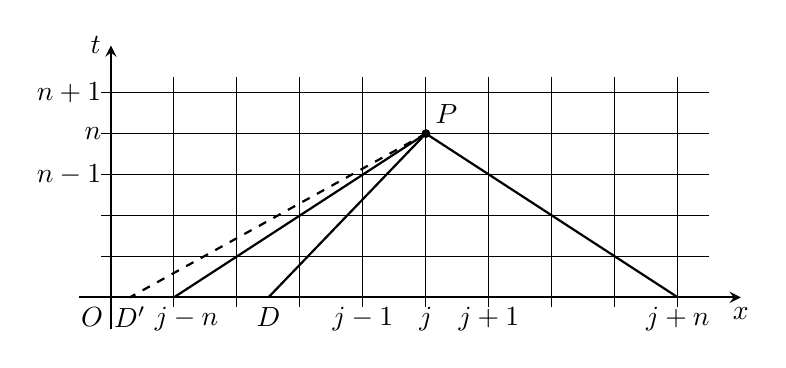
\begin{tikzpicture}[scale=0.8, >=stealth]
        % Grid
        \draw[xstep=1cm, ystep=0.65cm, black, thin] (-0.15,-0.15) grid (9.5,3.5);
        \draw[->, thick] (-0.5,0) -- (10,0) node[below] {$x$};
        \draw[->, thick] (0,-0.5) -- (0,4) node[left] {$t$};
        
        % Labels
        \node[left] at (0,3.25) {$n+1$};
        \node[left] at (0,2.6) {$n$};
        \node[left] at (0,1.95) {$n-1$};
        \node[below] at (-0.3,0) {$O$};
        
        \node[below] at (0.3,0) {$D'$};
        \node[below] at (1.2,0) {$j-n$};
        \node[below] at (2.5,0) {$D$};
        \node[below] at (4,0) {$j-1$};
        \node[below] at (5,0) {$j$};
        \node[below] at (6,0) {$j+1$};
        \node[below] at (9,0) {$j+n$};
        
        % Point P
        \fill (5,2.6) circle (2pt) node[above right] {$P$};
        
        % Lines
        \draw[thick] (5,2.6) -- (2.5,0);
        \draw[thick] (5,2.6) -- (1,0);
        \draw[thick, dashed] (5,2.6) -- (0.3,0);
        \draw[thick] (5,2.6) -- (9,0);
    \end{tikzpicture}
    \captionof{figure}{Lax-Wendroff 格式的依赖区域.}
\end{center}

根据格式\eqref{eq:lax-wendroff-c3}的定义知，为了确定 $u_j^n$，要用到格点函数值 $u_{j-1}^{n-1}$, $u_j^{n-1}$ 和 $u_{j+1}^{n-1}$；而为了得到这三个值, 又须用到 $u_{j-2}^{n-2}, u_{j-1}^{n-2}, \cdots, u_{j+2}^{n-2}$. 一直递推下去，为了确定 $u_j^n$，须用到初值 $u_0(x)$ 在区间 $[x_{j-n}, x_{j+n}]$ 上的所有格点值. 称\textcolor{red}{区间 $[x_{j-n}, x_{j+n}]$ 上的所有格点为差分格式解在点 $P(x_j, t_n)$ 处的依赖区域}.

由对流方程的精确解表达式 $u(x, t) = u_0(x - at)$ 可知，$D = x_j - at_n$ 为 $(x_j, t_n)$ 处精确解的依赖区域. \textcolor{red}{Courant-Friedrichs-Levy 条件 (CFL 条件) 就是要求 $D \in [x_{j-n}, x_{j+n}]$.}

Lax-Wendroff 格式稳定应满足
\begin{equation*}
    x_{j-n} \leq x_j - at_n \leq x_{j+n},
\end{equation*}
即 $a\lambda \leq 1$, 和前面得到的稳定性结果一致.

\begin{note}
    \begin{itemize}
    \item CFL 条件仅是一个描述性条件, 不能作为严格的稳定性判别准则来使用.
    \item 只需验证两层间的 CFL 条件是否满足即可.
    例如对于Lax-Wendroff 格式, 只需验证 $x_{j-1} \leq x_j - a\tau \leq x_{j+1}$，即 $a\tau\leq h \Leftrightarrow a\lambda \leq 1$ 即可.
\end{itemize}
\end{note}


\section{用特征线法构造差分格式}

特征线是研究双曲型方程定性理论的重要工具. 实际上, 它对构造双曲型方程的差分格式也很有帮助.

\noindent\textbf{Step 1:} 确定特征线方程. 对流方程 \eqref{eq:convection-3.1} 的特征线为
\begin{equation}
    L: \frac{\mathrm{d}x}{\mathrm{d}t} = a \implies x = at + x_0.
\end{equation}
沿特征线 $L$, 解 $u$ 恒为常数.

\noindent\textbf{Step 2:} 利用守恒性和插值方法构造差分格式. 记 $Q$ 为过点 $P=(x_j, t_{n+1})$ 的特征线与 $t=t_n$ 的交点, 则 $u(P)=u(Q)$. 如果 $Q$ 恰为网格节点, 则已获得差分格式. 如果它不是格点, 可通过给定在 $n$ 时间层上的格点函数值, 经插值方法得到 $u$ 在 $Q$ 点的近似值, 进而获得差分格式.

\subsection*{若干具体应用}

\textbf{情形 1.} 对固定的 $n$, 考虑时间层 $t_n$. 把该层的直线看成 $x$ 轴, $u(x, t_n)$ 看成 $x$ 的函数, 记为 $u^n(x)$. 简单的计算知点 $Q$的横坐标为 $x_j - a\tau$. 
\begin{enumerate}[法 1]
    \item 通过物理意义可知，$x_Q=x_j-a\tau$
    \item 由三角函数，$\tan\angle CPQ=k_{PQ}=a$.又$\tan\angle CPQ=\frac{|CP|}{|CQ|}=\frac{\tau}{|CQ|}$，故$|CQ|=a\tau$，从而$x_Q=x_j-a\tau$.
    \item 由方程$x_j-at_{n+1}=x_Q-at_n$，得$x_Q=x_j-a(t_{n+1}-t_n)=x_j-a\tau$.
\end{enumerate}
\begin{center}
    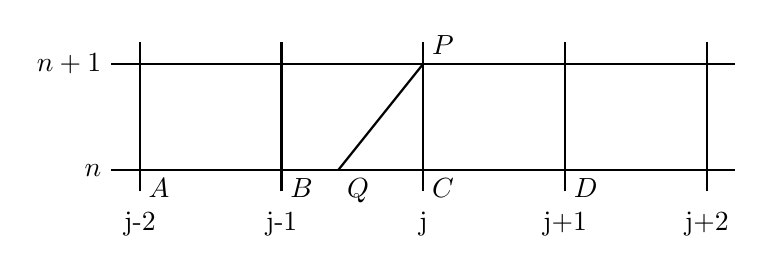
\begin{tikzpicture}[scale=0.9,x=2cm, y=1.5cm]
        \draw[thick] (-0.2, 0) -- (4.2, 0) node[left, pos=0] {$n$};
        \draw[thick] (-0.2, 1) -- (4.2, 1) node[left, pos=0] {$n+1$};
        
        \foreach \i/\text in {0/j-2, 1/j-1, 2/j, 3/j+1, 4/j+2} {
            \draw[thick] (\i, -0.2) -- (\i, 1.2);
            \node[below] at (\i, -0.3) {\text};
        }
        
        \node[below right, inner sep=3pt] at (0, 0) {$A$};
        \node[below right, inner sep=3pt] at (1, 0) {$B$};
        \node[below right, inner sep=3pt] at (2, 0) {$C$};
        \node[below right, inner sep=3pt] at (3, 0) {$D$};
        
        \node[above right, inner sep=3pt] at (2, 1) {$P$};
        \coordinate (Q) at (1.4, 0);
        \node[below right, inner sep=3pt] at (Q) {$Q$};
        
        \draw[thick] (2, 1) -- (Q);
    \end{tikzpicture}
\end{center}
以$x_{j-1}$ (对应点 $B$) 和 $x_j$ (对应点 $C$)作线性插值, 相应的插值函数为
\begin{equation}
    u^n(x) = \frac{x_j - x}{h} u_{j-1}^n + \frac{x - x_{j-1}}{h} u_j^n.
\end{equation}
把 $Q$ 点横坐标代入有
\begin{equation*}
    \begin{aligned}
        u^n(Q) &= u^n(x_j - a\tau) \\
        &\approx \frac{x_j - (x_j - a\tau)}{h} u_{j-1}^n + \frac{(x_j - a\tau) - x_{j-1}}{h} u_j^n \\
        &= a\lambda u_{j-1}^n + (1-a\lambda)u_j^n,
    \end{aligned}
\end{equation*}
于是得差分格式:
\begin{equation}
    u_j^{n+1} = a\lambda u_{j-1}^n + (1-a\lambda)u_j^n, \quad \lambda = \tau/h.
\end{equation}
它恰为前面介绍的迎风格式.

\noindent\textbf{情形 2.} 如果以$B,C,D$三点的格点函数值作二次插值, 则仿照上述推导可得 Lax-Wendroff 格式.\par
\noindent\textbf{情形 3.} 如果以$B,D$两点的格点函数值作线性插值, 则仿照上述推导可得 Lax-Friedrichs 格式.\par
\noindent\textbf{情形 4.} 如果以$A,B,C$三点的格点函数值作二次插值, 则得如下 Beam-Warming 格式:
\begin{equation}
    u_j^{n+1} = u_j^n - a\lambda(u_j^n - u_{j-1}^n) - \frac{a\lambda}{2}(1-a\lambda)(u_j^n - 2u_{j-1}^n + u_{j-2}^n).
\end{equation}
该格式又称为二阶迎风格式. 该格式的稳定性条件为 $a\lambda \leq 2$.\par
\noindent\textbf{情形 5. p阶迎风格式} \par
\noindent\textbf{Step 1. 向后Newton插值.} 我们需要知道Newton插值$N_hu(x_Q)$的大小.\par
记$u(x_Q)=u(x-\alpha h)=E^{-\alpha}u(x)$，$\nabla  u_j=u_j-u_{j-1}$，则
\begin{equation*}
    \nabla = I-E^{-1},E^{-1}=I-\nabla
\end{equation*}
那么代入上式即得
\begin{equation*}
    u(x_Q)=(I-\nabla)^\alpha u(x)=\sum_{k=0}^\infty \binom{\alpha}{k}(-1)^k \nabla^k u(x).
\end{equation*}
\noindent\textbf{Step 2. 截断 }特别地，如果考虑Newton插值，则其取值正好等于上述展开在$p$处的截断，即
\begin{equation*}
    N_hu(x_Q)=u_j-\mathrm{C}_\alpha^1\nabla u_j+\mathrm{C}_\alpha^2\nabla^2 u_j-\cdots + (-1)^p \mathrm{C}_\alpha^p \nabla^p u_j.
\end{equation*}
其中$\alpha=a\lambda$.\par

通过CFL条件可知$p$阶迎风格式的稳定性为$a\lambda\leq p$.'




\noindent\textbf{情形 6.} 如果以点 $Q$ 所在的空间网格区间端点作线性插值来获得 $u(Q)$ 的近似值, 则可导出如下修正的迎风格式:
\begin{equation}
    u_j^{n+1} = \{a\lambda\} u_{j-[a\lambda]-1}^n + (1-\{a\lambda\}) u_{j-[a\lambda]}^n,
\end{equation}
式中, $[x]$ 表示不超过 $x$ 的最大整数, 而 $\{x\} = x - [x]$. 该格式是无条件稳定的.

除迎风型格式外, 前面介绍的其他差分格式都可自然推广到偏微分方程组情形. 例如, 对于问题
\begin{equation}
    \begin{cases}
        \partial_t \boldsymbol{u} + \boldsymbol{A} \partial_x \boldsymbol{u} = \boldsymbol{0}, \\
        t=0, \boldsymbol{u} = \boldsymbol{u}_0(x),
    \end{cases}
\end{equation}
相应的 Lax-Friedrichs 格式为
\begin{equation}
    \frac{\boldsymbol{u}_j^{n+1} - \frac{1}{2}(\boldsymbol{u}_{j-1}^n + \boldsymbol{u}_{j+1}^n)}{\tau} + \boldsymbol{A} \frac{\boldsymbol{u}_{j+1}^n - \boldsymbol{u}_{j-1}^n}{2h} = \boldsymbol{0}.
\end{equation}

\section{一阶变系数双曲型方程的差分法}

考虑如下一阶变系数双曲型方程:
\begin{equation}\label{eq:variable-coefficient-hyperbolic}
    \begin{cases}
        u_t + a(x,t)u_x = 0, \\
        t=0, u=u_0(x).
    \end{cases}
\end{equation}
现在来建立求解该问题的差分方法.

\textbf{方法 1. 冻结系数法.}

将方程在网格点 $(x_j, t_n)$ 的系数 $a(x,t)$ 冻结为常数 $a(x_j, t_n)$ 而得
\begin{equation*}
    u_t + a(x_j, t_n)u_x = 0,
\end{equation*}
然后用前面介绍的常系数情形的差分格式在 $(x_j, t_n)$ 处进一步离散, 比如, 设 $a(x_j, t_n) > 0$, 用迎风格式离散可得
\begin{equation}\label{eq:upwind-variable}
    \frac{u_j^{n+1} - u_j^n}{\tau} + a(x_j, t_n)\frac{u_j^n - u_{j-1}^n}{h} = 0.
\end{equation}

\begin{figure}[htbp]
    \centering
    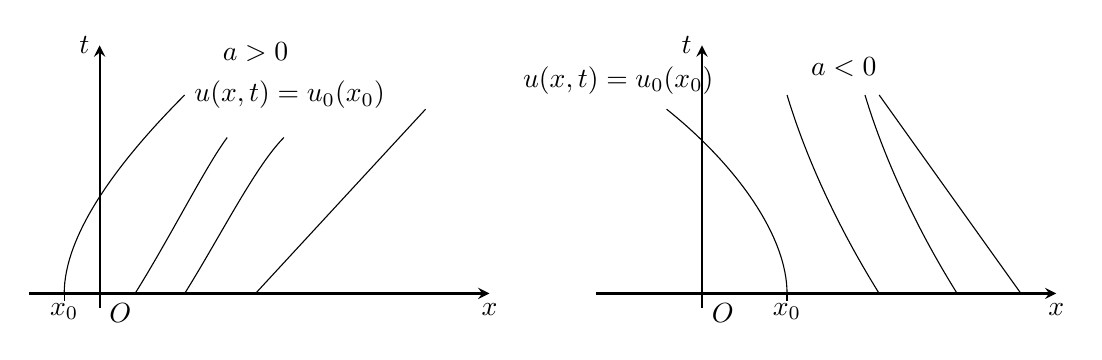
\begin{tikzpicture}[scale=0.9, >=stealth]
        % Left figure (a > 0)
        \begin{scope}
            \draw[->, thick] (-1,0) -- (5.5,0) node[below] {$x$};
            \draw[->, thick] (0,-0.2) -- (0,3.5) node[left] {$t$};
            \node[below right] at (0,0) {$O$};
            
            \draw (-0.5,-0.1) -- (-0.5,0) node[below] {$x_0$};
            \draw (-0.5,0) .. controls (-0.5,0.8) and (0.2,1.8) .. (1.2,2.8);
            \node[right] at (1.2,2.8) {$u(x,t) = u_0(x_0)$};
            
            \draw (0.5,0) .. controls (1.0,0.8) and (1.5,1.8) .. (1.8,2.2);
            \draw (1.2,0) .. controls (1.7,0.8) and (2.2,1.8) .. (2.6,2.2);
            \draw (2.2,0) -- (4.6,2.6);
            
            \node at (2.2, 3.4) {$a > 0$};
        \end{scope}
        
        % Right figure (a < 0)
        \begin{scope}[xshift=8.5cm]
            \draw[->, thick] (-1.5,0) -- (5,0) node[below] {$x$};
            \draw[->, thick] (0,-0.2) -- (0,3.5) node[left] {$t$};
            \node[below right] at (0,0) {$O$};
            
            \draw (1.2,-0.1) -- (1.2,0) node[below] {$x_0$};
            \draw (1.2,0) .. controls (1.2,0.8) and (0.5,1.8) .. (-0.5,2.6);
            \node[left] at (0.3,3) {$u(x,t) = u_0(x_0)$};
            
            \draw (2.5,0) .. controls (2.0,0.8) and (1.5,1.8) .. (1.2,2.8);
            \draw (3.6,0) .. controls (3.1,0.8) and (2.6,1.8) .. (2.3,2.8);
            \draw (4.5,0) -- (2.5,2.8);
            
            \node at (2.0, 3.2) {$a < 0$};
        \end{scope}
    \end{tikzpicture}
    \caption{特征曲线.}
    \label{fig:characteristics}
\end{figure}

\textbf{方法 2. 特征线方法.}

问题\eqref{eq:variable-coefficient-hyperbolic}过 $(\bar{x}_0, \bar{t}_0)$ 的特征线方程为
\begin{equation}\label{eq:characteristic-variable}
    (L): \begin{cases}
        \frac{\mathrm{d}x}{\mathrm{d}t} = a(x,t), \\
        t = \bar{t}_0, x = \bar{x}_0.
    \end{cases}
\end{equation}
故知
\begin{equation}
    u_j^{n+1} \approx u(x_j, t_{n+1}) = u(x(t_n; x_j, t_{n+1}), t_n).
\end{equation}

从而问题的关键是如何近似求解 $x(t_n; x_j, t_{n+1})$ (后文简记为 $x(t_n)$). 一旦得到它, 可以通过插值的方法, 求出 $u$ 在这点的近似值, 进而获得差分方程. 为此, 对特征线方程 \eqref{eq:characteristic-variable} 在 $[t_n, t_{n+1}]$ 积分, 并注意到 $t = t_{n+1}$ 时, $x = x_j$, 可有
\begin{equation*}
    x_j - x(t_n) = \int_{t_n}^{t_{n+1}} a(x,t) \,\mathrm{d}t.
\end{equation*}

\begin{enumerate}[(1)]
    \item 右矩形公式.
    \begin{equation*}
        x_j - x(t_n) \approx \tau a(x_j, t_{n+1}) \implies x(t_n) \approx x_j - \tau a(x_j, t_{n+1}).
    \end{equation*}
    \item 左矩形公式.
    \begin{equation*}
        x_j - x(t_n) \approx \tau a(x(t_n), t_n) \implies \text{求得 } x(t_n) \text{ 的近似值.}
    \end{equation*}
    \item 梯形公式.
    \begin{equation*}
        x_j - x(t_n) \approx \frac{\tau}{2}(a(x_j, t_{n+1}) + a(x(t_n), t_n)) \implies \text{求得 } x(t_n) \text{ 的近似值.}
    \end{equation*}
\end{enumerate}

\textbf{核心思想：}利用特征线方程, 将偏微分方程数值求解转化为常微分方程数值求解.

\subsection{差分格式的稳定性分析}

现在用能量方法研究差分格式的稳定性. 设 $a(x,t) > 0$, 考虑求解问题 \eqref{eq:variable-coefficient-hyperbolic} 的差分格式 \eqref{eq:upwind-variable} 的稳定性. 该格式可重写为
\begin{equation*}
    u_j^{n+1} = u_j^n - \lambda a_j^n(u_j^n - u_{j-1}^n),
\end{equation*}
式中, $a_j^n = a(x_j, t_n)$, $\lambda = \tau/h$ 为网格比.

\textbf{若干假设:}
\begin{enumerate}[(1)]
    \item $a(x,t)$ 在 $\mathbb{R} \times [0, +\infty)$ 连续可微, 且存在常数 $M > 0$ 满足
    \begin{equation}\label{eq:assumption-a}
        \sup_{x,t} [|a(x,t)| + |a_x(x,t)|] \leq M < +\infty.
    \end{equation}
    \item 初值满足
    \begin{equation*}
        \int_{-\infty}^{+\infty} u_0^2(x) \,\mathrm{d}x < +\infty.
    \end{equation*}
\end{enumerate}

设
\begin{equation}\label{eq:CFL-variable}
    \lambda \max_j a_j^n \leq 1.
\end{equation}
在差分方程两侧同乘以 $u_j^{n+1}$, 再利用 Cauchy-Schwarz 不等式可知
\begin{equation*}
    \begin{aligned}
        (u_j^{n+1})^2 &\leq (1 - \lambda a_j^n)u_j^n u_j^{n+1} + \lambda a_j^n u_{j-1}^n u_j^{n+1} \\
        &\leq \frac{1 - \lambda a_j^n}{2} \{ (u_j^n)^2 + (u_j^{n+1})^2 \} + \frac{\lambda a_j^n}{2} \{ (u_{j-1}^n)^2 + (u_j^{n+1})^2 \},
    \end{aligned}
\end{equation*}
即
\begin{equation*}
    (u_j^{n+1})^2 \leq (1 - \lambda a_j^n)(u_j^n)^2 + \lambda a_j^n(u_{j-1}^n)^2.
\end{equation*}

令 $\|u^n\|_h^2 = \sum_{j=-\infty}^\infty h (u_j^n)^2$. 经推导可知对任意 $T > 0$, 当 $n\tau \leq T$ 时, 成立
\begin{equation*}
    \|u^n\|_h^2 \leq (1 + M\tau)^n \|u^0\|_h^2 \leq e^{MT} \|u^0\|_h^2.
\end{equation*}
因此, 若条件 \eqref{eq:CFL-variable} 成立时, 格式 \eqref{eq:upwind-variable} 是稳定的.

\section{一阶双曲型方程初边值问题的差分法}

\subsection{边值条件提法}

构造一阶双曲型方程初边值问题的差分方法, 很有技巧性. 实际上, 如何对一阶双曲型方程提合理的边值条件都非常有讲究.

现以如下方程为例来具体说明:
\begin{equation*}
    u_t - u_x = 0, \quad 0 < x < 1, \quad t > 0,
\end{equation*}
初值条件为
\begin{equation*}
    u(x,0) = f(x).
\end{equation*}
问题: 如何提合适的边值条件?

\begin{figure}[htbp]
    \centering
    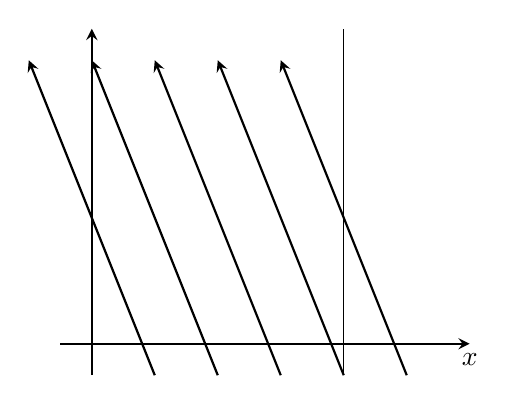
\begin{tikzpicture}[scale=0.8, >=stealth]
        % Axes
        \draw[->, thick] (-0.5,0) -- (6,0) node[below] {$x$};
        \draw[->, thick] (0,-0.5) -- (0,5); % t axis
        \draw (4,-0.5) -- (4,5); % x=1 line
        
        % Characteristics x+t=c or dx/dt=-1
        % so x = -t + c
        \foreach \c in {0, 1, 2, 3, 4} {
            \draw[->, thick] (\c + 1, -0.5) -- (\c - 1, 4.5);
        }
    \end{tikzpicture}
    \caption{边值条件提法.}
\end{figure}

此时应该沿着流体流动方向, 在流体入口处提边值条件:
\begin{equation*}
    x = 1, \quad u = g(t).
\end{equation*}

\textbf{数学直观描述：}为保证问题的适定性, 如果特征线先碰到初值线, 则提初值条件, 如果先碰到边值线, 则对该线提边值条件.

\subsection{差分格式}

将空间区域 $[0,1]$ 作 $J$ 等分, 则 $x$ 方向的步长为 $h$, 可仿照构造一阶双曲型方程初值问题差分格式的思想来处理相应的初边值问题.

\textbf{方法 1: 迎风格式.}
\begin{equation*}
    \begin{cases}
        \frac{u_j^{n+1} - u_j^n}{\tau} - \frac{u_{j+1}^n - u_j^n}{h} = 0, \quad 0 < j < J, \\
        u_J^n = g(t_n) = g_n, \\
        u_j^0 = f(x_j) = f_j.
    \end{cases}
\end{equation*}
该格式的精度为 $O(\tau + h)$.

\textbf{$x = 0$ 处的网格点赋值：}
设想 $x = 0$ 处也满足双曲型方程, 则使用迎风格式离散可得
\begin{equation*}
    \frac{u_0^{n+1} - u_0^n}{\tau} - \frac{u_1^n - u_0^n}{h} = 0.
\end{equation*}

\textbf{方法 2: 蛙跳格式.}
\begin{equation}\label{eq:leapfrog}
    \frac{u_j^{n+1} - u_j^{n-1}}{2\tau} - \frac{u_{j+1}^n - u_{j-1}^n}{2h} = 0, \quad 0 < j < J.
\end{equation}
该格式精度为 $O(\tau^2 + h^2)$. 同样地, 它在 $x = 0$ 处的信息无法知道. 有两个解决方法:
\begin{enumerate}[(1)]
    \item 均匀化法. 作均匀化假设 $\frac{u_0^n + u_2^n}{2} = u_1^n$. 但这样做将会出现回流现象, 导致格式失真.
    \item 迎风格式法. 在 $x = 0$ 处离散时用迎风格式
    \begin{equation*}
        u_0^{n+1} = u_0^n + \lambda(u_1^n - u_0^n)
    \end{equation*}
    或格式
    \begin{equation*}
        u_0^{n+1} = u_0^{n-1} + \lambda \left( u_1^n - \frac{1}{2}(u_0^{n+1} + u_0^{n-1}) \right).
    \end{equation*}
\end{enumerate}

\textbf{例: 用蛙跳格式数值求解问题}
\begin{equation*}
    \begin{cases}
        u_t - u_x = 0, \quad 0 < x < 1, \ 0 < t < 0.5, \\
        t = 0, \quad u_0(x) = f(x), \\
        x = 1, \quad u = g(t),
    \end{cases}
\end{equation*}
其中, $f(x), g(t)$ 由精确解 $u(x,t) = e^{-\alpha(x+t)}$ 确定 ($\alpha > 0$ 为参数).

内部点的离散格式为 \eqref{eq:leapfrog}, 即
\begin{equation*}
    u_j^{n+1} = u_j^{n-1} + \lambda(u_{j+1}^n - u_{j-1}^n), \quad \lambda = \tau/h.
\end{equation*}

\begin{figure}[htbp]
    \centering
    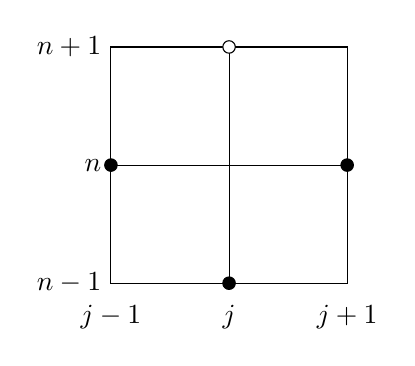
\begin{tikzpicture}[scale=1.5, >=stealth]
        % Grid
        \draw (-1, -1) rectangle (1, 1);
        \draw (-1, 0) -- (1, 0);
        \draw (0, -1) -- (0, 1);
        
        % Labels
        \node[left] at (-1, 1) {$n+1$};
        \node[left] at (-1, 0) {$n$};
        \node[left] at (-1, -1) {$n-1$};
        \node[below] at (-1, -1.1) {$j-1$};
        \node[below] at (0, -1.1) {$j$};
        \node[below] at (1, -1.1) {$j+1$};
        
        % Points
        \filldraw[black] (-1, 0) circle (1.5pt); % (j-1, n)
        \filldraw[black] (1, 0) circle (1.5pt);  % (j+1, n)
        \filldraw[black] (0, -1) circle (1.5pt); % (j, n-1)
        \filldraw[fill=white, draw=black] (0, 1) circle (1.5pt); % (j, n+1)
    \end{tikzpicture}
\end{figure}

蛙跳格式的节点示意图如上，即用三个黑点处的值求白点处的值，显然白点达不到区域的左右边界，因而对本问题，需要给出左边界的处理方法，这里选取均匀化法和迎风格式法. 计算开始时需要 $n=0$ 和 $n=1$ 时间层的结果以进行迭代. 为了聚焦左边界点处不同离散化方法引起的不同效应，使用精确解来获得这些值.

根据理论分析稳定的充要条件是 $\lambda = \tau/h < 1$，计算中取 $h = 0.02$, $\tau = 0.01$. 均匀化法是用左边界处的值构造平均得到的，因而当精确解在左边界处变化较大时，相应的数值解应该会出现较大的偏差. 为了观察这种效应，我们逐渐增大参数 $\alpha$，相应的数值结果表现如下:

\begin{enumerate}[(1)]
    \item 当 $\alpha$ 增大时，均匀化法的计算结果在真实解附近振荡，而且随时间增大，这种振荡越明显，这是因为此时真实解在左端的变化更大. 这种非物理性振荡恰好符合均值的特性. 与此不同的是，迎风格式法的计算结果与真实解很好地吻合.
    \item 如果比较误差极值的话，迎风格式法也明显优于均匀化法.
\end{enumerate}

\section{二阶双曲型方程的差分方法}

二阶双曲型方程的弦振动方程的初值问题为
\begin{equation} \label{eq:wave-equation}
    \begin{cases}
        u_{tt} - a^2 u_{xx} = 0, \ x \in \mathbb{R}, t > 0, \\
        t=0, \ u = u_0(x), \ u_t = u_1(x),
    \end{cases}
\end{equation}
式中 $a > 0$ 为常数.

构造它的差分格式有两种方法.

\textbf{方法 1. 数值微分方法.}

将 $u_{tt}$ 和 $u_{xx}$ 用中心差商离散即得 ($n=1, 2, \cdots, \ j=0, \pm 1, \cdots$)
\begin{equation} \label{eq:wave-finite-difference}
    \frac{u_j^{n+1} - 2u_j^n + u_j^{n-1}}{\tau^2} - a^2 \frac{u_{j+1}^n - 2u_j^n + u_{j-1}^n}{h^2} = 0.
\end{equation}
易得该差分方程的截断误差为 $O(\tau^2 + h^2)$. 对该格式的稳定性分析留作练习.

\textbf{方法 2. 高阶方程化为一阶方程组法.}

令 $v = u_t$, $w = a u_x$, 则由 \eqref{eq:wave-equation} 可知
\begin{equation*}
    \begin{cases}
        v_t - a w_x = 0, \\
        a v_x - w_t = 0.
    \end{cases}
\end{equation*}

如记 $\boldsymbol{u} = [v, w]^T$, 则上式即为
\begin{equation*}
    \boldsymbol{u}_t -
    \begin{bmatrix}
        0 & a \\
        a & 0
    \end{bmatrix}
    \boldsymbol{u}_x = \boldsymbol{0}.
\end{equation*}
对该方程组可以构造多个差分格式离散.

\vspace{1ex}
现在对初值条件进行离散. 对于 $0$ 时间层, 自然有 $u_j^0 = u_0(x_j)$. 对于 $1$ 时间层, 如果将 $u_t$ 用前向差商离散, 则得
\begin{equation*}
    \frac{u_j^1 - u_j^0}{\tau} = u_t(x_j, 0) = u_1(x_j).
\end{equation*}
该方法只有一阶精度.

\begin{figure}[htbp]
    \centering
    \begin{tikzpicture}[scale=1]
        % Axes
        \draw[->, thick] (-1,0) -- (6,0) node[right] {$x$};
        \draw[->, thick] (2.5,-1.5) -- (2.5,3.5) node[above] {$t$};
        % Grid
        \draw (-0.5,0) rectangle (5.5,3);
        \draw (-0.5,1) -- (5.5,1);
        \draw (-0.5,2) -- (5.5,2);
        \draw (1,0) -- (1,3);
        \draw (4,0) -- (4,3);
        % Virtual grid dashed
        \draw[dashed] (-0.5,-1) rectangle (5.5,0);
        \draw[dashed] (1,-1) -- (1,0);
        \draw[dashed] (4,-1) -- (4,0);
    \end{tikzpicture}
    \caption{虚拟网格示意图}
    \label{fig:virtual-grid}
\end{figure}

另一种方法是引进虚拟网格 $(x_j, -\tau)$ 及格点函数 $u_j^{-1}$ (见图 \ref{fig:virtual-grid}).

在 $(x_j, 0)$ 处假设满足弦振动方程并用中心差商离散, 对 $u_t$ 也使用中心差商离散, 则得
\begin{equation*}
    \begin{cases}
        \frac{u_j^1 - u_j^{-1}}{2\tau} = u_t(x_j, 0) = u_1(x_j), \\[1ex]
        \frac{u_j^1 - 2u_j^0 + u_j^{-1}}{\tau^2} - a^2 \frac{u_{j+1}^0 - 2u_j^0 + u_{j-1}^0}{h^2} = 0,
    \end{cases}
\end{equation*}
由此可有
\begin{equation*}
    u_j^1 = u_0(x_j) + \tau u_1(x_j) + \frac{1}{2}(a\lambda)^2 \{u_{j+1}^0 - 2u_j^0 + u_{j-1}^0 \}.
\end{equation*}

以上结果也可由 Taylor 展开得到:
\begin{equation*}
    \begin{aligned}
        u_j^1 &\approx u(x_j, \tau) = u(x_j, 0) + \tau u_t(x_j, 0) + \frac{1}{2}\tau^2 u_{tt}(x_j, 0) + O(\tau^3) \\
        &= u_0(x_j) + \tau u_1(x_j) + \frac{1}{2}a^2\tau^2 u_{xx}(x_j, 0) + O(\tau^3),
    \end{aligned}
\end{equation*}
故取
\begin{equation*}
    u_j^1 = u_0(x_j) + \tau u_1(x_j) + \frac{1}{2}(a\lambda)^2 \{u_0(x_{j+1}) - 2u_0(x_j) + u_0(x_{j-1}) \}.
\end{equation*}
这个格式具有二阶精度, 和差分方程 \eqref{eq:wave-finite-difference} 的精度吻合.